\documentclass[12pt]{article}

%%%%%%%%%%%%%%%%%%%%%%% Don't change anything in here. This space is called the preamble, it is where you tell the computer to load the proper LaTeX packages to perform the math and formatting desired. 

\usepackage{graphicx}
\graphicspath{ {./images/} }
\usepackage{hyperref}
\hypersetup{
    colorlinks=true,
    linkcolor=blue,
    filecolor=magenta,      
    urlcolor=blue,
}
\usepackage[utf8]{inputenc}
\usepackage{physics} 
\usepackage{siunitx} 
\usepackage{enumerate} 
\usepackage{pgfplots}
\usepackage{pgfplotstable}
\usepackage{tikz,pgfplots}
\usepackage{amsmath}  
\usepackage{textcomp}
	
\usepackage{geometry}
 \geometry{
 a4paper,
 total={170mm,257mm},
 left=20mm,
 top=20mm,
 }

\pgfplotsset{compat=1.14}
%%%%%%%%%%%%%%%%%%%%%%%%% Again, Don't change anything Above %%%%%%%%%%%%%%%%%%%%

\begin{document}

\title{GitHub: a Practical Introduction} %Title should be concise and to the point  
\author{Fran\c{c}ois Gerard} %Your name first


\date{\today}  % This will automatically put today's date in the report

\maketitle  %this command makes the title

%%%% to use this template, please copy-paste the entire thing into a new document and save it so you have it!

%%%%% If you want to omit something in this lab, place a % sign to the left of it and it won't show up on the lab, like this line!

\begin{abstract} 
	This is a very short and practical introduction to GitHub intended to future RAs and co-authors. Most of commands for GitHub are very well documented online and you should have no problems to find them, but what can be sometimes tricky is understanding how to start using GitHub. I will briefly describe the main concepts of GitHub and try to illustrate the most important tools using one practical example. After reading this introduction you should be able to use GitHub in a project straight away. I recommend several website for specific tools along the way, but the most complete reading is \href{https://git-scm.com/book/en/v2}{Pro Git - Everything You Need to Know About Git} %\cite{1}. 
\end{abstract}

\section{Introduction}
	 
    In the following sections I will guide you through (i) editing an existing project in Git and (ii) creating a project of your own and transferring it to Git.
    
    %note the cite above. That is an in text citation. By putting citations in your bibliography, you can cite in text simply using the \cite{} command and putting the number of the citation in the {} 
    
\section{GitHub Basics}

\subsection{Distributed Version Control System}
	As you probably know, GitHub is a Version Control System (VCS) -- it stores in repositories (often called repos) all the versions from your project's history that you 'committed' (we'll see what commit means in GitHub, but you can think of it as saving a version of your program). However, a key feature of GitHub that differentiates it from older VCSs is that it is a Distributed VCS. This means that GitHub not only stores a version of your project on its cloud service (called remote repo), but also every participant of a project stores the entire history of that project on their computers. So besides storing the current version of the project that you are working on (called the working directory), you also store a Git repository on your computer with the project's history (called the local repo). 

	In figure 1 below, the Version Database is what we call the 'remote repo.' The Files in Computer A and in the Computer B are the "working directories" and the Version Database in each computer are the 'local repos.' Local repos, or .git repos, are by default hidden in your computer, so you'll only see your working directory. Being a Distributed VCS allows GitHub to be (i) incredibly fast, since it doesn't have to access the internet to access a project's history; (ii) independent from your internet connection, for the same reason, and (iii) very safe, since every user serves essentially as a backup of the project's history.
	\vspace{0.3 in}
	
	\begin{figure}[t]
	\caption{Distributed Version Control System}
	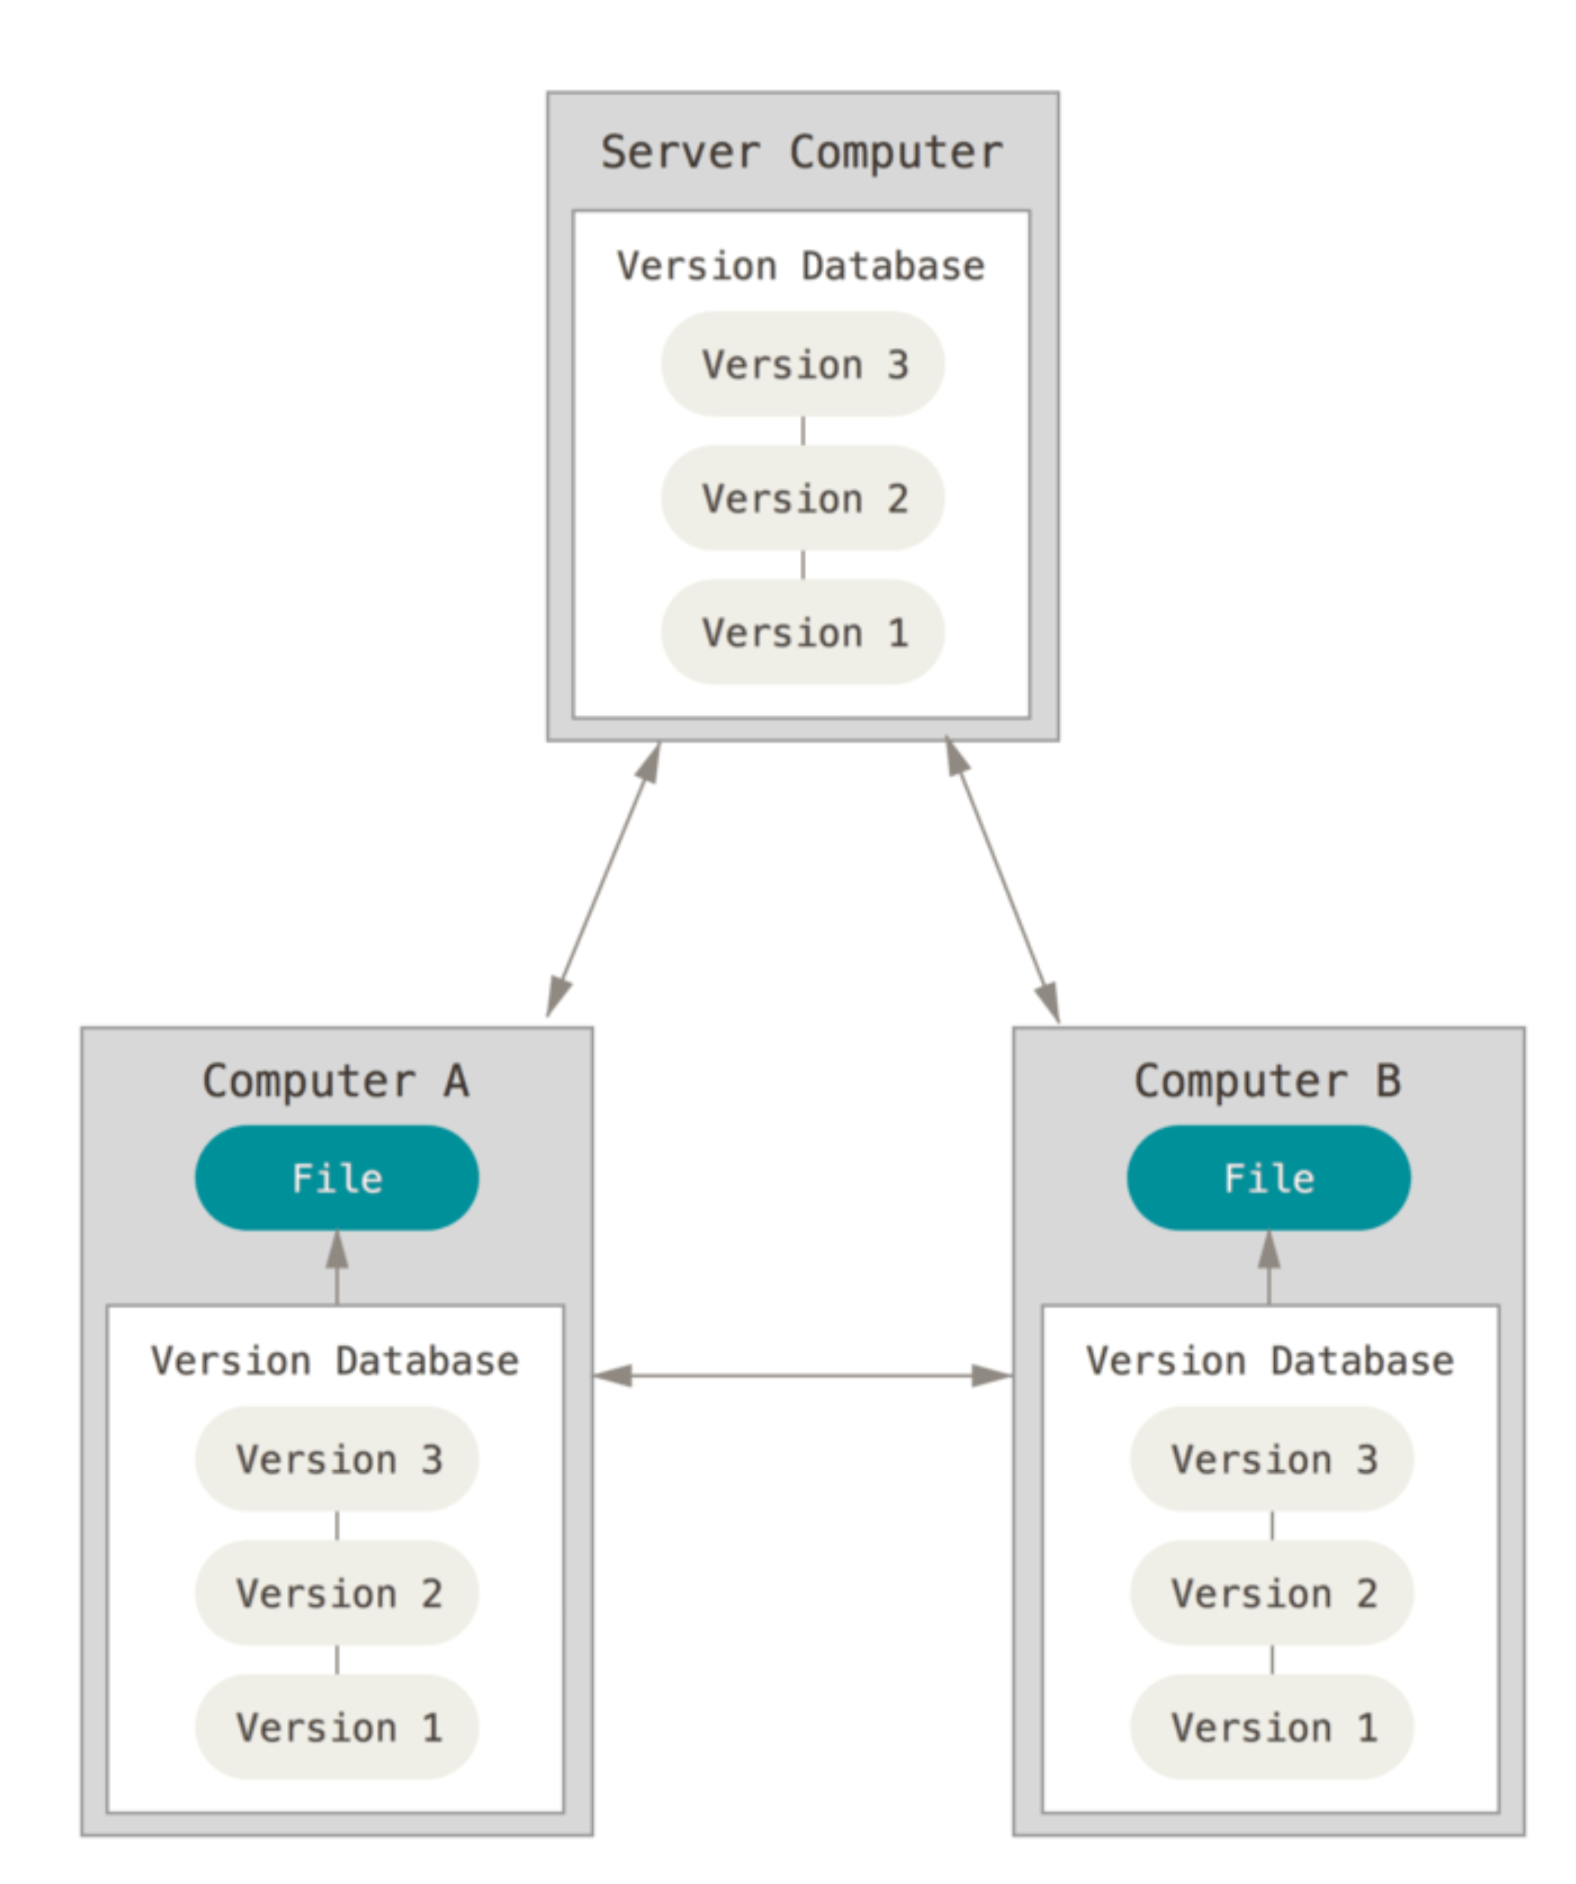
\includegraphics[scale=0.5]{figure1}
	\centering
    \end{figure}

\subsection{Git Setup}
    \begin{description}
    \item[$\bullet$] First step: install Git. You can find instructions \href{https://git-scm.com/book/en/v2/Getting-Started-Installing-Git}{here}. 
    \item[$\bullet$] Second step: create an account on \href{https://github.com}{GitHub}
    \item[$\bullet$] Third step (optional): setup your identity. Go to your terminal and type the following commands:
    \newline
    \newline
    \indent \$git config --global user.name "John Doe"
    \newline
    \newline
    \indent \$git config --global user.email johndoe@example.com \\
    
    Don\textquotesingle t actually copy the \$ symbol, this is standard notation to let you know this command should be run in the terminal. If you need any help to understand a command, you can type the git help $<$verb$>$. For instance: \\
    \\
    \indent \$git help config
    
    \end{description}

\section{Joining a Project: Cloning an Existing Repo}

    This section guides you through an example on how to join an existing project, probably that your Professor, or co-author, already began. This will be useful to introduce some concepts and Git commands. It will also be all that RAs will need to know 90\% of the times.
    
\subsection{Clone a repo}

    To clone a repository means that you are reaching out to a remote repository and copying nearly all data that the server has into a new local repo in your computer. Let's illustrate this with an example:
    \begin{description}
    \item[$\bullet$] First step: access the url of the \href{https://github.com/luigicaloi/GitShortIntro}{remote repo}.
    \item[$\bullet$] Second step: Open terminal
    \item[$\bullet$] Third step: Go to the directory where you want your repo to be: \\ \\
    \indent \$ cd /Users/username/documents 
    
    \item[$\bullet$] Fourth step: Go to the \href{https://github.com/luigicaloi/GitShortIntro}{remote repo}, click on clone or download and copy that link displayed. Then, on your terminal, clone the repository with git clone $<$ulr$>$   \\
    
    \indent \$ git clone  https://github.com/luigicaloi/GitShortIntro.git
    \vspace{0.1 in}
    \end{description}
    This will create a GitShortIntro directory with a working copy of the latest version of the project. It also stores a .git directory (the local repo) inside it, which is hidden. For more info, see \href{https://help.github.com/articles/cloning-a-repository/}{this}.
    
    \subsection{Staging Modified Files}
    If you open the new GitShortIntro directory, you\textquotesingle ll see that there are only two files, 'AllReaders.tex' and 'Test.do,' and one folder 'GitHub\_a\_Practical\_Introduction.' Your task is simple: open the 'AllReaders.tex' file and include your name at the end of the list of all readers.
    
    Now that you have made changes to the working directory, let\textquotesingle s see what is your status in Git. Change the directory in the terminal for the one from your new project. For instance:
    
    \vspace{0.1 in}
    \indent \$ cd /Users/username/documents/GitShortIntro
    \newline
    \newline
    and write the following command on the terminal:
    \newline
    \newline
    \indent \$ git status
    \begin{figure}[h]
	\caption{Git status}
	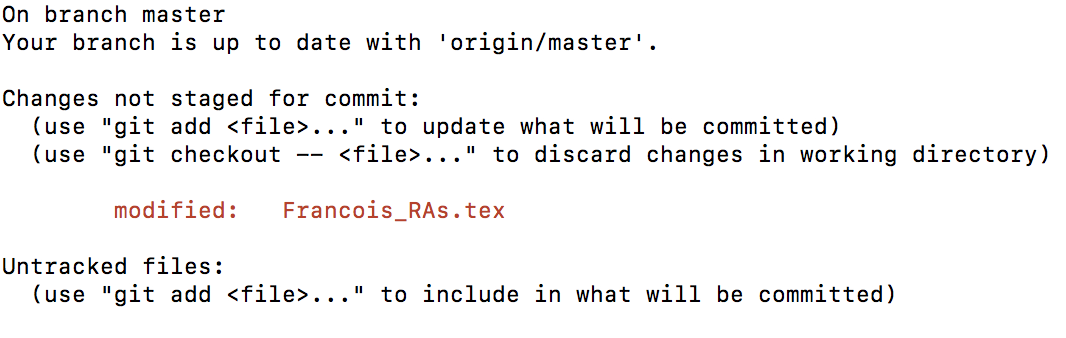
\includegraphics[scale=0.5]{figure2}
	\centering
    \end{figure}
    \vspace{0.1 in}
    Don\textquotesingle t worry about the branch message, we\textquotesingle ll see what that is in section \hyperref[sec:branching]{Git Branching}. GitHub realizes that your local repo is different from your working directory, it realized that you made changes to the 'Francois\_RAs.tex' file and shows it under 'Changes to be committed.' Our goal here is to make sure that your local repo also saves those changes (we?ll take care of the remote repo in the next subsection). You first need to tell GitHub what documents you want to save the changes in the local repo with the following command:
    \newline
    \newline
    \indent \$ git add AllReaders.tex
    \newline
    \newline
    Now run git status again and you\textquotesingle ll see:
    \newline
    \begin{figure}[h]
	\caption{Git status}
	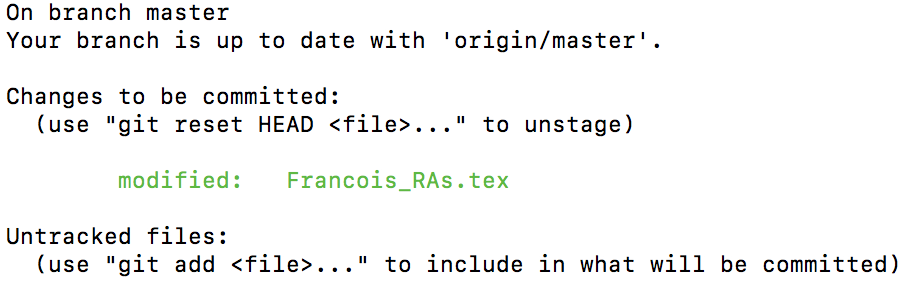
\includegraphics[scale=0.5]{figure3}
	\centering
    \end{figure}
    \vspace{0.1 in}
    \subsection{Committing a Modified File}
    AllReaders.tex is now under the 'Changes to be committed.' Next, we need to 'commit' those changes. Committing is telling GitHub to take a snapshot of your project in the working directory and save it, with the changes, to your local repository. In other words, you are 'saving' your latest changes to the git repo.
    See \href{https://git-scm.com/docs/git-commit}{this} for more details. The command to commit changes is:\\
    \\
    \indent \$ git commit -m 'A message explaining your changes to the project'
    \subsection{Unmodifying a Modified File}
    If you accidentally modified a file, or regretted the changes, and wants to revert it back to how it was when you last committed (the local repo's last snapshot), you can run the following command: \\
    \\
    \indent \$git checkout -- $<$file$>$ \\
    \\
    However, be careful, the changes you had made and not committed will be completely deleted.
    \subsection{Pushing to Your Remotes}
    \label{sec:pushing}
    So you have already (i) cloned all the data from the remote repo and created a local repo; (ii) modified your working directory and (iii) added and committed your changes from your working directory to your local repo (the .git repository). We'll now update your changes to the remote repo. This can be done with the following command: \\
    \\
    \indent \$git push origin master \\
    \\
    Or more generally \\
    \\
    \indent \$git push $<$remote$>$ $<$branch$>$ \\
    \\
    'origin' is the automatic name that GitHub assigns to the remote repository. 'master' is the branch in the remote repo, but don\textquotesingle t worry about it yet, it will make sense after we see \hyperref[sec:branching]{Git Branching}. Git push uploads the changes from your local repo to your remote repo. Now your working directory, your local repo and your remote repo are all on the same stage.
    \section{Creating a Repo}
    \subsection{Creating an Empty Repo}
    In the last section we saw how to clone a repo, make changes to your local repo and push it back to the remote. In this section we will simply see how to create an empty remote repo, then you can follow the workflow from Section 3 to add your files to it.
    \begin{description}
    \item[$\bullet$] First step: Go to GitHub\textquotesingle s website and login.
    \item[$\bullet$] Second step: On any page, click the + button on the upper right part of the screen and then click New repository 
    \item[$\bullet$] Third step: Choose the name of your repo and click Create repository. 
    \end{description}
    For more options, see \href{https://help.github.com/articles/creating-a-new-repository/}{this}
    \subsection{Adding an Existing Project to Your New Repo}
    To add an existing project to the new remote repo, we will first create a local repo, add the existing project to it, commit the changes and push it to the empty remote repo. 
    \begin{description}
    \item[$\bullet$] First step: Change the current working directory to the desired local\textquotesingle s project dir. \\
    \\
    \indent \$cd /Users/username/newrepo \\
    \item[$\bullet$] Second step: Initialize a local git repository in your current directory \\  
    \\
    \indent \$git init \\
    \item[$\bullet$] Third step: Add the files for your new repo 
    \item[$\bullet$] Fourth step: Commit the new files, which creates a snapshot of how they are now and save it to the local repo
    \item[$\bullet$] Fifth step: Go back to your remote repo on GitHub\textquotesingle s website and copy the remote repository URL.
    \item[$\bullet$] Sixth step: Add the new remote repo from your terminal
    \indent \$git remote add origin $<$remote repository URL$>$
    \item[$\bullet$] Seventh step: Your local repo is now connected to your remote repo. Push your changes to your remote repo as we saw in \hyperref[sec:pushing]{Pushing to Your Remote}.
    \end{description}
    For more details and options, see \href{https://help.github.com/articles/adding-an-existing-project-to-github-using-the-command-line/}{this}.
    \section{Branching and Merging}
    In this section we will see the two concepts that are most important for collaborative work -- branching and merging.
    \subsection{Git Branching}
    \label{sec:branching}
    The easiest way to understand branches is to think about the repo as a series of commits. When you create a repo, GitHub automatically creates a branch called master. This branch is simply a pointer to the last commit of your project. In figure 3 bellow, for instance, the master branch is pointing to the third and last commit (C2). \\
    \begin{figure}[h]
	\caption{Branch Master}
	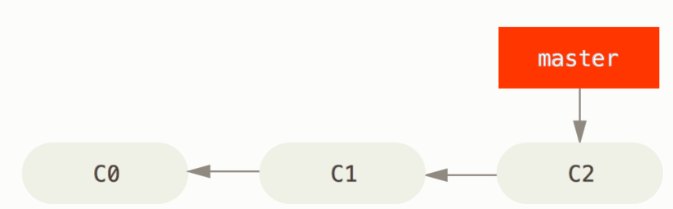
\includegraphics[scale=0.5]{figure4}
	\centering
    \end{figure} 
    \vspace{0.2 in}
    Now let\textquotesingle s say that you need to make changes to your project for a new submission, but you don\textquotesingle t want to change the original code yet. You  can create a new branch, called testing, with the following command \vspace{0.2 in}\\
    \\
    \indent\indent \$git branch testing \\
    \\
    \begin{figure}[h]
	\caption{New Branch}
	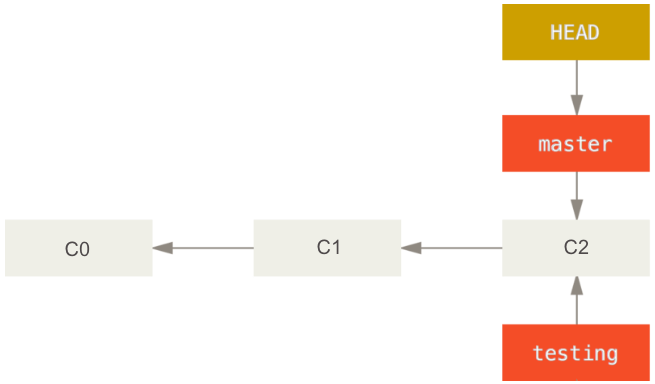
\includegraphics[scale=0.5]{figure5}
	\centering
    \end{figure} 
    \vspace{0.2 in}
    Now the two branches are pointing to the last commit (see figure 5). The HEAD pointer shows which branch you are currently working in your local repo.
    The following command switches control to the testing branch so that you can make the new changes to your project. \\
    \\
    \indent\indent \$git checkout testing \\
    \\
    Now if you make changes to your project and commit them, your project history will look like Figure 6. Note that the master branch is still pointing to commit C2.
    \vspace{0.2 in}
    \begin{figure}[h]
	\caption{New Branch}
	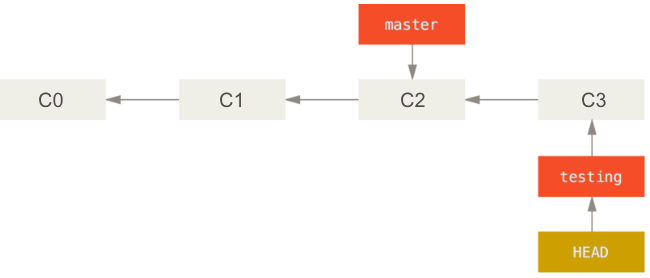
\includegraphics[scale=0.5]{figure6}
	\centering
    \end{figure} 
    \vspace{0.2 in}
    The good thing is that if we decide that the new ideas were bad, we can simply go back to the master branch with \\
    \indent\indent\$git checkout master \\
    With this, all the files on your working directory go back to how they were when you made the last push in your master branch (C2). \\
    Another scenario that illustrates why it is good to make new changes in branches is when a journal asks you to make a change some details to a paper in which you\textquotesingle ve been making drastic changes. You can easily go back to your 'master' version (assuming this is the one you submitted to the journal), make changes to it, and then go back to your 'testing' branch to continue working on the big changes.
    \subsection{Git Merging}
    Following from last subsection\textquotesingle s example, let\textquotesingle s suppose that while you made changes to the 'testing' branch, someone else had to make urgent changes to the master branch. For that, this person created a 'hotfix' branch. The history of your project now looks like this: 
    \vspace{0.3 in}
    \begin{figure}[h]
	\caption{New Branch}
	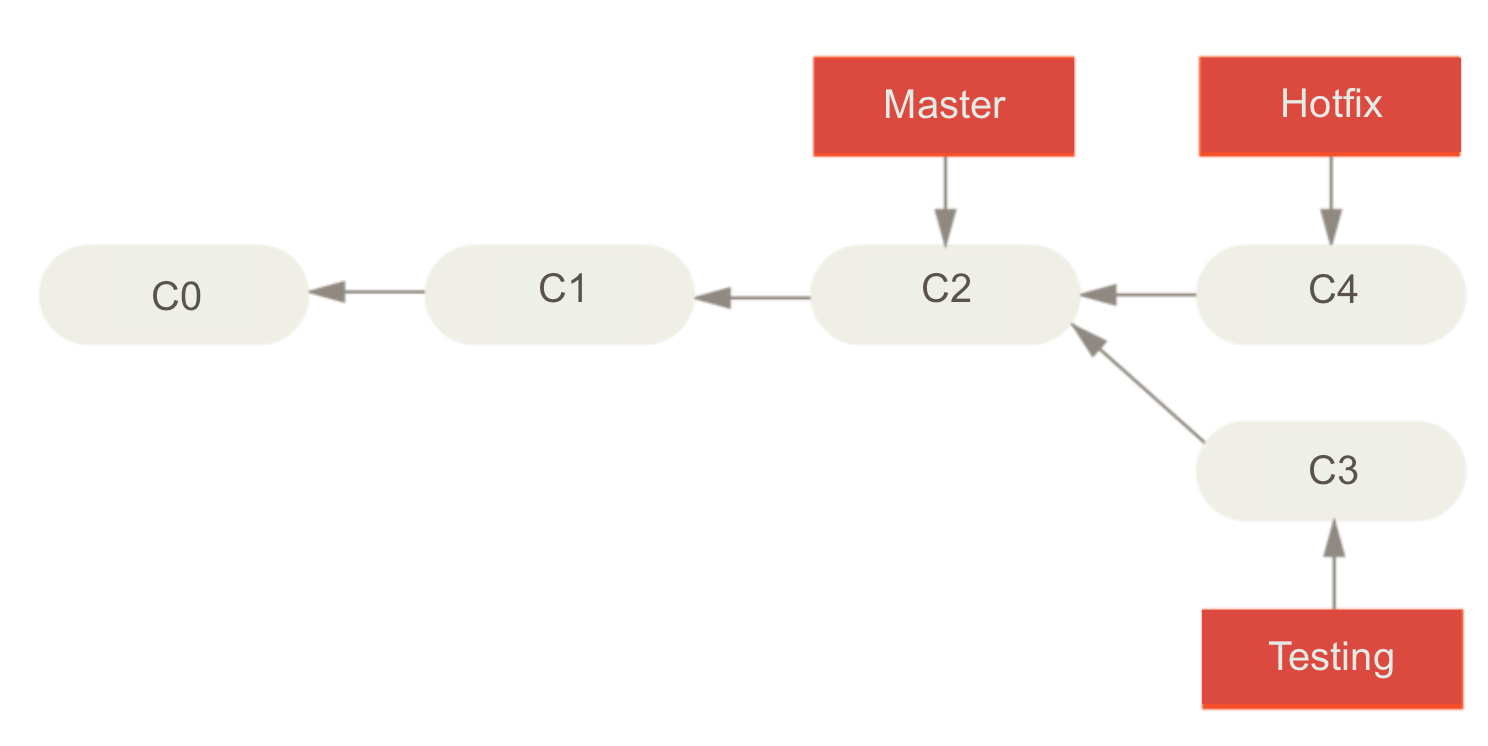
\includegraphics[scale=0.5]{figure7}
	\centering
    \end{figure} 
    \vspace{5 in}
    Now let\textquotesingle s say we finished the changes in the hotfix branch and we are ready to merge the master branch with the hotfix branch. This can be done with the following command:\\
    \\
    \indent\indent \$git checkout master \\ 
    \\
    \indent\indent \$git merge hotfix \\
    \\
    And we would see the following message: \\
    \begin{figure}[h]
	\caption{New Branch}
	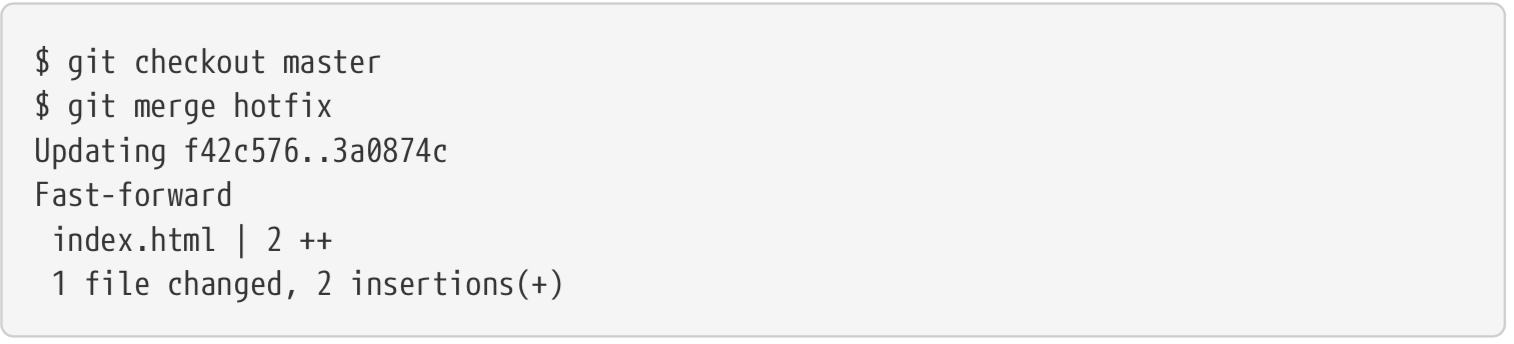
\includegraphics[scale=0.5]{figure8}
	\centering
    \end{figure} 
    \vspace{0.2 in}
    Because the commit C4 from the hotfix branch was directly ahead of C3, GitHub can simply 'fast-forward' the master branch and change the pointer from C3 to C4. Since the hotfix branch and the master branch now point to the same commit, we can delete the hotfix branch: \\
    \\
    \indent\indent \$git branch -d hotfix 
    \subsubsection{Merging conflicts}
    Things are a bit more complicated when you are trying to merge two branches that are not directly related. If some change made in the hotfix branch conflicts with changes made in the testing branch, GitHub won't be able to complete the merge and will ask your help to decide which version it should keep for that specific change. The first step would be to try merging both branches. \\
     \\
    \indent\indent \$git merge testing \\
    \\
    We would then check in which files there was a merge conflict with git status  \\
    \begin{figure}[h]
	\caption{New Branch}
	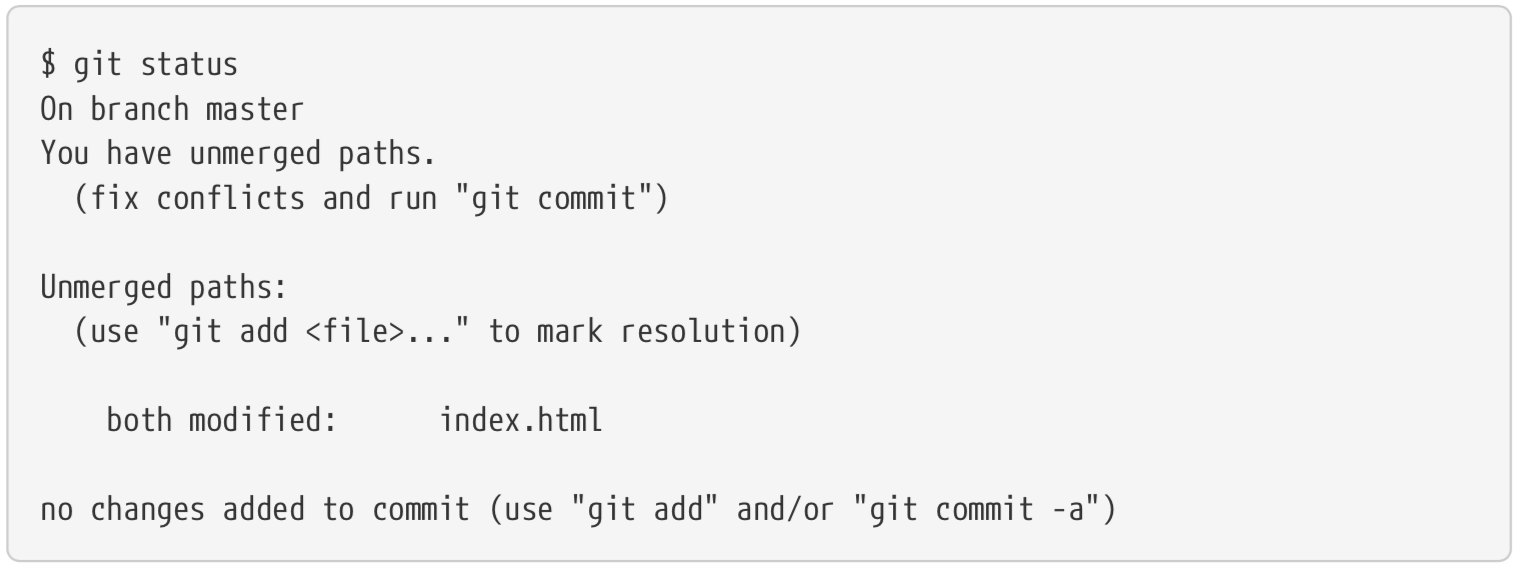
\includegraphics[scale=0.5]{figure9}
	\centering
    \end{figure} 
    \vspace{0.2 in}
    Any file with a merge conflict would be under unmerged paths. To solve the conflicts, we first need to open the files in a text editor. GitHub adds conflict resolution markers in it so that we can solve the conflict manually. The section of the file that must be solved looks like this: \\
    \begin{figure}[h]
	\caption{New Branch}
	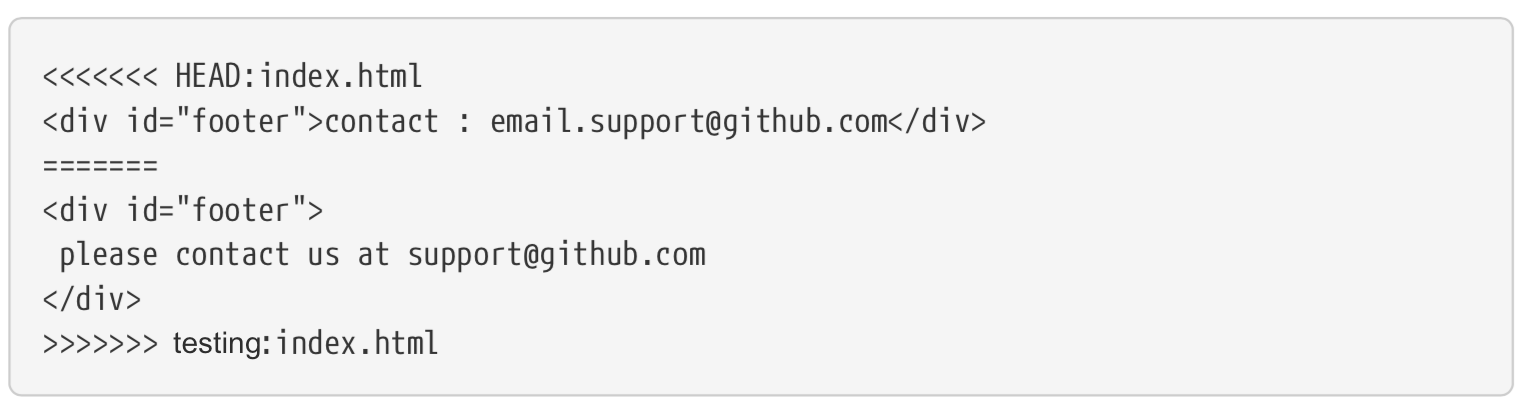
\includegraphics[scale=0.5]{figure10}
	\centering
    \end{figure} \\
    \vspace{0.2 in}
    The changes made to the master branch are under $<<<<<<<<$ HEAD:index.html and above the ======= lines, because HEAD was pointing to the master branch (you were in the master branch). Everything bellow $<$div id="footer"$>$ and above  $>>>>>>>$ testing:index.html was in the testing branch. You can manually solve this issue by keeping the version you prefer, or a combination of both. Of course, delete the conflict signals from GitHub. \\
    \indent For instance, one way to solve this issue would be to substitute the entire block with this: \\
    \begin{figure}[h]
	\caption{New Branch}
	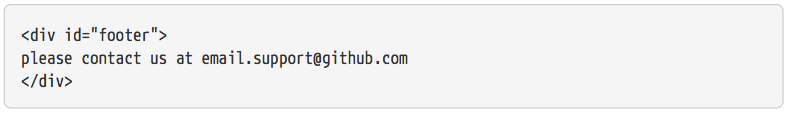
\includegraphics[scale=0.5]{figure11}
	\centering
    \end{figure} \\
    Once you're done solving the conflicts, the next step would be to let Git know these files are solved by running git add in the terminal
    \newline
    \newline
    \indent\indent \$git add document
    \newline
    \newline
    You can then commit your changes and finish merging the two branches.
    For more details, please see \href{https://git-scm.com/book/en/v2/Git-Branching-Basic-Branching-and-Merging}{this}.
    When merging branches that are not directly linked, instead of just moving the branch pointer forward, GitHub will create a new commit that includes the changes in hotfix and testing. Your new commit history will look like this: \\
    \begin{figure}[h]
	\caption{New Branch}
	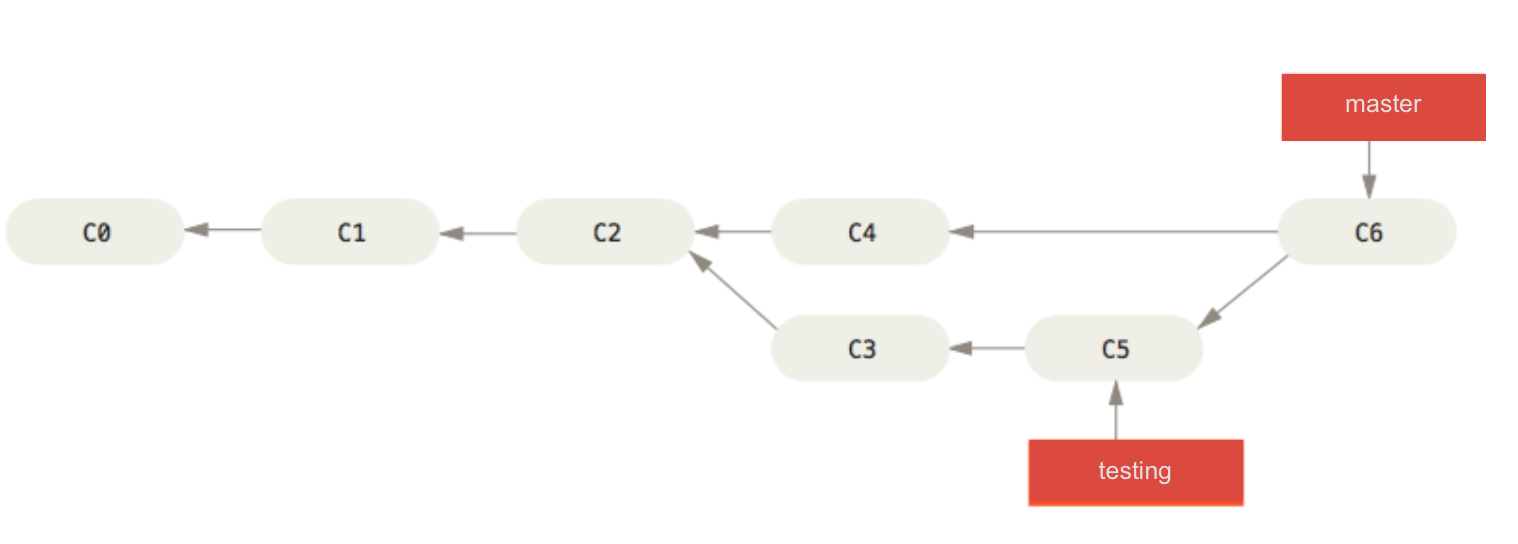
\includegraphics[scale=0.5]{figure12}
	\centering
    \end{figure} 
    \\
    Branching and merging allow us to understand better what was going on with the push command in \hyperref[sec:pushing]{Pushing to Your Remote}. We saw how to push a local repository to a remote one with the command git push $<$remote$>$ $<$branch$>$, but we told you to not pay attention to what was the branch part of it. Just like our local repo, the remote repo can have multiple branches (they usually follow the same structure as our local repo). The $<$branch$>$ command is simply telling Git to what branch of our remote repo we want to push our changes. Second, it might have seemed like Git magically sent the data to the remote repo and made both be on the same stage. What if there are three people working on the same branch and pushing their changes to the branch in the remote repository? The push command is implicitly merging the local and remote branches. Therefore, if there are multiple people pushing to the same branch, we might need to fix merge conflicts to decide what changes to keep.
    \section{Using GitDesktop}
    While using the terminal can be very good to work on GitHub, the GitDesktop app is useful for visualizing what changed in a new push. 
    \begin{description}
    \item[$\bullet$] First, download GitDesktop  \href{https://desktop.github.com/}{here}.
    \item[$\bullet$] Second, add your local repository to the GitHub Desktop by clicking on File and Add Local Repository.
    \item[$\bullet$] Third, on the left of your screen, choose GitShortIntro as your current repository and master as your current branch.
    \item[$\bullet$] Fourth, click on pull origin to make sure that your GitHub Desktop is up to date with the remote repo.
    \item[$\bullet$] Fifth, Under your current repository, click on "history."
    \end{description}
    This is a list of the commits to that repository to the master branch on the GitShortIntro remote repository. You can click in one of the commits to see what changes were made. In red are the deleted lines and in green that ones that were added. \\
    \begin{figure}[t]
	\caption{GitHub Desktop}
	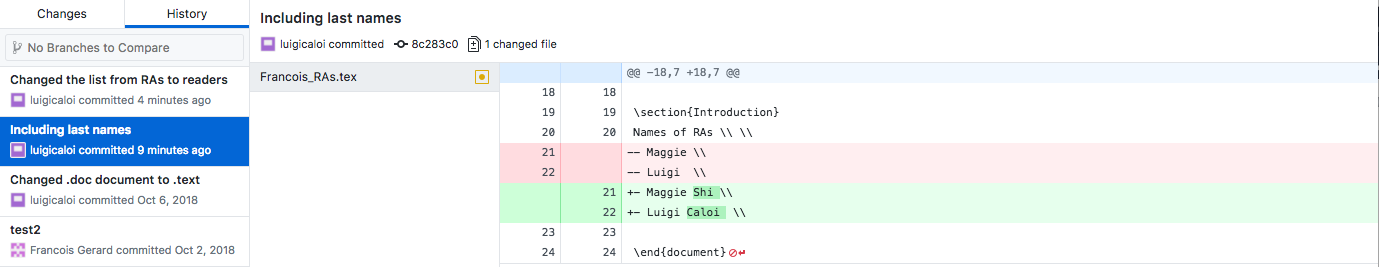
\includegraphics[scale=0.5]{figure13}
    \end{figure} 
    \end{document}
    
    
    

%%%%%%%%%%%%%%%%%%%%%%%%%%%%%%%%%%%%%%%%%%%%%%%%%%%%%%%%%%%%%%%%%%%%%%%%%%%%%%%%%%%%%
%%%% This is the Bibliography where you will cite your sources used in the paper %%%%

%\begin{thebibliography}{0}

	%Each item starts with a \bibitem{} command and the details thereafter.
	
	%\bibitem{1} Cite your first source here
	%\bibitem{2} Cite another source
	
    %%% The 1,2 etc. are used to cite in text. See up in the intro for an example
    %%% When you want to cite in your cite, type in \cite{} wherever you want
%\end{thebibliography}
    


\end{document}
